% Demo paper: information-theoretic perception for robot decision making.
% Embedded with {% tex_file "/assets/papers/example-paper.tex" %}.
\documentclass[11pt]{article}
\usepackage[margin=1in]{geometry}
\usepackage[utf8]{inputenc}
\usepackage[T1]{fontenc}
\usepackage{amsmath,amssymb}
\usepackage{microtype}
\usepackage{graphicx}
\usepackage{booktabs}
\usepackage{enumitem}
\usepackage{tikz}
\usetikzlibrary{arrows.meta,positioning,shapes.geometric,fit,backgrounds,calc}
\definecolor{teal}{HTML}{2AA198}
\definecolor{orange}{HTML}{D07A3F}
\definecolor{blue}{HTML}{61AFEF}
\definecolor{green}{HTML}{98C379}
\definecolor{purple}{HTML}{C678DD}
\definecolor{papergray}{HTML}{5C6370}
\usepackage[colorlinks=true,urlcolor=blue,linkcolor=black,citecolor=blue]{hyperref}
\setlength{\parskip}{0.4em}

\title{Learning to Perceive, Perceiving to Act:\\
  An Information-Theoretic View of Robot Decision Making}
\author{Shivaram Kumar Jagannathan\\
  \small{\texttt{shivaram.jagannathan [at] outlook [dot] com}}}
\date{\today}

\begin{document}
\maketitle

\begin{abstract}
Robot decision making is only as reliable as the information supplied by
perception. This paper develops a complementary view of learning-based
robotics in which deep visual models, information theory, and physical
inductive biases work together. A perception system should not merely predict
what is visible; it should estimate which uncertainties matter for the next
decision and choose observations that reduce them. We formalise this idea with
mutual information, Bayesian belief updates, and expected information value.
We then connect these objectives to physics-informed representation learning,
where geometry, dynamics, and conservation laws regularise learned models.
Optimisation-based controllers, search-based planners, and learned policies
are treated as downstream decision mechanisms that can all benefit from a
better belief state. The result is a view of perception as an active,
decision-aware inference process rather than a passive front end.
\end{abstract}

\section{Introduction}
\label{sec:intro}

Robotic systems must infer hidden state from incomplete, noisy, and often
adversarial observations before they can choose a useful action. A camera does
not reveal mass, friction, contact mode, or whether an occluded object will
move when pushed. A learned policy can be expressive, while a symbolic planner
can be interpretable and compositional, but both still depend on the quality of
the state or belief supplied to them.

The choice of decision mechanism does not remove this dependence. Optimisation,
search, sampling, and learned policies provide different ways to convert beliefs
into actions, but each inherits the blind spots of its perceptual interface. Our
claim is therefore narrow: perception should be trained and evaluated by how it
changes downstream decisions, not only by pixel-level or object-level accuracy.

The central question is therefore:
\begin{quote}
  Which observation should a robot seek next, and how much will that
  observation improve the decisions it can make?
\end{quote}

Figure~\ref{fig:loop} gives the proposed loop. A deep model extracts a
representation from sensor data, an information-theoretic objective identifies
decision-relevant uncertainty, and a planner or controller chooses an action
that both pursues the task and improves the next belief update.

\begin{figure}[ht]
\centering
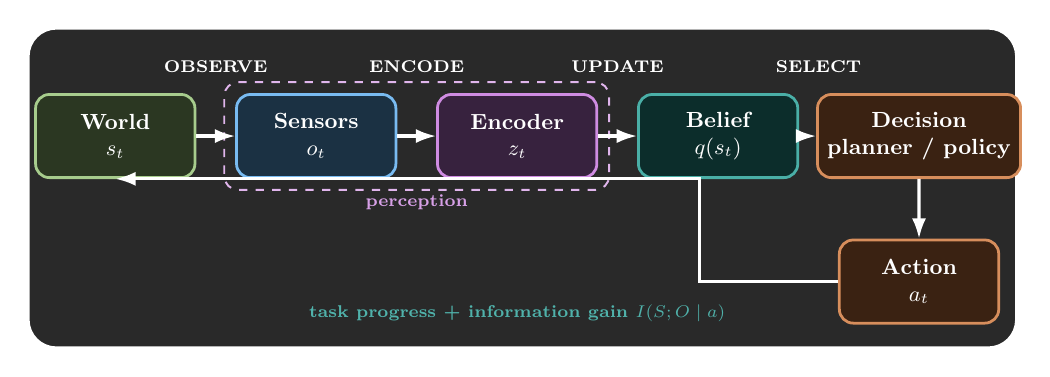
\begin{tikzpicture}[
  scale=.88, transform shape,
  every node/.style={font=\footnotesize},
  box/.style={rounded corners=5pt, draw=#1!85, fill=#1!28!black,
    text=white, align=center, minimum height=12mm, minimum width=23mm,
    line width=1pt, font=\small\bfseries, inner sep=4pt},
  arr/.style={-{Latex[length=2.6mm,width=1.8mm]}, line width=1.15pt, white!72},
  ann/.style={font=\scriptsize\bfseries, text=white!72}
]
\begin{scope}[on background layer]
  \fill[black!84, rounded corners=10pt] (-1.25,-3.05) rectangle (13.0,1.55);
  \draw[white!12, rounded corners=10pt, line width=.7pt]
    (-1.25,-3.05) rectangle (13.0,1.55);
\end{scope}
% top pipeline
\node[box=green]  (world)    at (0,0)    {World\\$s_t$};
\node[box=blue]   (sensor)   at (2.9,0)  {Sensors\\$o_t$};
\node[box=purple] (encoder)  at (5.8,0)  {Encoder\\$z_t$};
\node[box=teal]   (belief)   at (8.7,0)  {Belief\\$q(s_t)$};
\node[box=orange] (decision) at (11.6,0) {Decision\\planner / policy};
% bottom action
\node[box=orange] (action)   at (11.6,-2.1) {Action\\$a_t$};

% forward arrows
\draw[arr] (world)    -- (sensor);
\draw[arr] (sensor)   -- (encoder);
\draw[arr] (encoder)  -- (belief);
\draw[arr] (belief)   -- (decision);
\draw[arr] (decision) -- (action);

% labels above the pipeline (never on the arrows)
\node[ann] at (1.45,1.0)  {OBSERVE};
\node[ann] at (4.35,1.0)  {ENCODE};
\node[ann] at (7.25,1.0)  {UPDATE};
\node[ann] at (10.15,1.0) {SELECT};

% return path below, clear of everything
\draw[arr, white!55]
  (action.west) -- ++(-2.0,0) |- (world.south);
\node[ann, text=teal!82] at (5.8,-2.55)
  {task progress + information gain $I(S;O\mid a)$};

% soft grouping under perception
\begin{scope}[on background layer]
  \node[fit=(sensor)(encoder), rounded corners=5pt, inner sep=4pt,
    draw=purple!55, dashed, line width=.7pt] {};
\end{scope}
\node[ann, text=purple!70] at (4.35,-0.95) {perception};
\end{tikzpicture}
\caption{Perception and decision making as one loop. The robot can choose
actions for task progress and for information gain, while the downstream
planner, controller, or policy operates on an explicitly uncertain belief.}
\label{fig:loop}
\end{figure}

\begin{figure}[ht]
\centering
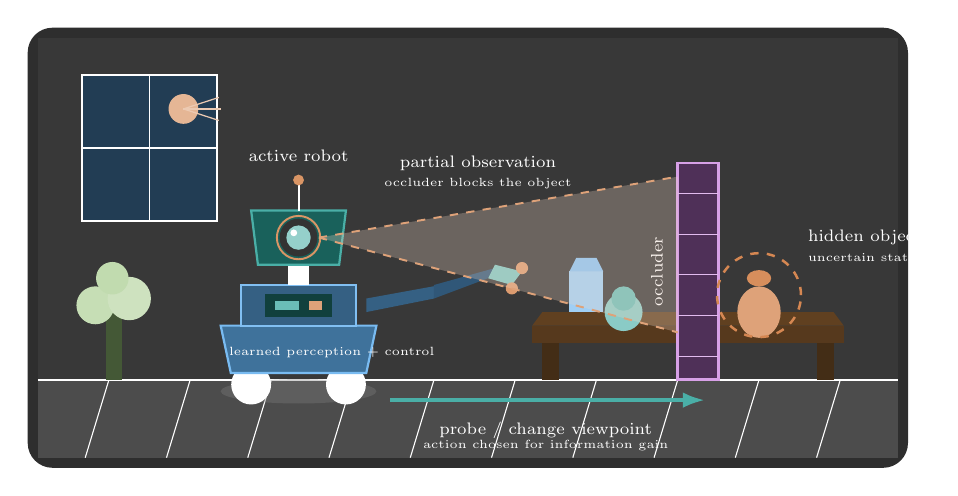
\begin{tikzpicture}[
  scale=.86, transform shape,
  every node/.style={font=\footnotesize},
  lab/.style={font=\scriptsize, text=white!88},
  sublab/.style={font=\tiny, text=white!65}
]
% ---- room ----
\fill[black!82, rounded corners=9pt] (-0.45,-0.95) rectangle (12.55,5.55);
\fill[black!78] (-0.3,-0.8) rectangle (12.4,5.4);           % wall
\fill[black!70] (-0.3,-0.8) -- (12.4,-0.8) -- (12.4,0.35) -- (-0.3,0.35) -- cycle; % floor
\draw[white!18, line width=.6pt] (-0.3,0.35) -- (12.4,0.35);
% floor grid
\foreach \x in {0.4,1.6,2.8,4.0,5.2,6.4,7.6,8.8,10.0,11.2}
  \draw[white!8, line width=.4pt] (\x,-0.8) -- (\x+0.35,0.35);
% window + light
\fill[blue!35!black] (0.35,2.7) rectangle (2.35,4.85);
\draw[white!35, line width=.8pt] (0.35,2.7) rectangle (2.35,4.85);
\draw[white!25, line width=.5pt] (1.35,2.7) -- (1.35,4.85);
\draw[white!25, line width=.5pt] (0.35,3.775) -- (2.35,3.775);
\fill[orange!55] (1.85,4.35) circle (0.22);
\foreach \a in {-18,0,18}
  \draw[orange!40, line width=.45pt] (1.85,4.35) -- ++(\a:0.55);
% plant
\fill[green!45!black] (0.7,0.35) rectangle (0.95,1.35);
\fill[green!55] (0.55,1.45) circle (0.28);
\fill[green!48] (1.05,1.55) circle (0.32);
\fill[green!60] (0.8,1.85) circle (0.24);

% ---- table ----
\fill[brown!45!black] (7.0,0.9) rectangle (11.6,1.15);
\fill[brown!35!black] (7.15,0.35) rectangle (7.4,0.9);
\fill[brown!35!black] (11.2,0.35) rectangle (11.45,0.9);
\fill[brown!50!black] (7.0,1.15) -- (11.6,1.15) -- (11.45,1.35) -- (7.15,1.35) -- cycle;
% visible objects on table
\fill[blue!60] (7.55,1.35) rectangle (8.05,1.95);
\fill[blue!75] (7.55,1.95) -- (8.05,1.95) -- (7.95,2.15) -- (7.65,2.15) -- cycle;
\fill[teal!55] (8.35,1.35) circle (0.28);
\fill[teal!70] (8.35,1.55) circle (0.18);

% ---- tall occluder ----
\fill[purple!40!black] (9.15,0.35) rectangle (9.75,3.55);
\draw[purple!70, line width=1pt] (9.15,0.35) rectangle (9.75,3.55);
\foreach \y in {0.7,1.3,1.9,2.5,3.1}
  \draw[purple!50, line width=.4pt] (9.15,\y) -- (9.75,\y);
\node[lab, rotate=90, anchor=south] at (9.05,1.95) {occluder};

% ---- hidden object behind occluder ----
\fill[orange!70] (10.35,1.35) ellipse (0.32 and 0.38);
\fill[orange!85] (10.35,1.85) ellipse (0.18 and 0.12);
\draw[orange!90, dashed, line width=.9pt] (10.35,1.6) circle (0.62);
\node[lab, anchor=west] at (10.95,2.45) {hidden object};
\node[sublab, anchor=west] at (10.95,2.15) {uncertain state};

% ---- robot (detailed) ----
% shadow
\fill[black!50, opacity=0.35] (3.55,0.18) ellipse (1.15 and 0.18);
% wheels
\fill[white!25] (2.85,0.28) circle (0.28);
\fill[white!15] (2.85,0.28) circle (0.12);
\fill[white!25] (4.25,0.28) circle (0.28);
\fill[white!15] (4.25,0.28) circle (0.12);
\draw[white!40, line width=.7pt] (2.85,0.28) circle (0.28);
\draw[white!40, line width=.7pt] (4.25,0.28) circle (0.28);
% chassis
\fill[blue!65!black] (2.55,0.45) -- (4.55,0.45) -- (4.7,1.15) -- (2.4,1.15) -- cycle;
\draw[blue!85, line width=.8pt] (2.55,0.45) -- (4.55,0.45) -- (4.7,1.15) -- (2.4,1.15) -- cycle;
\fill[blue!55!black] (2.7,1.15) rectangle (4.4,1.75);
\draw[blue!80, line width=.7pt] (2.7,1.15) rectangle (4.4,1.75);
% chest panel
\fill[teal!40!black] (3.05,1.28) rectangle (4.05,1.62);
\fill[teal!70] (3.2,1.38) rectangle (3.55,1.52);
\fill[orange!70] (3.7,1.38) rectangle (3.9,1.52);
% neck + head
\fill[white!30] (3.4,1.75) rectangle (3.7,2.05);
\fill[teal!60!black] (2.95,2.05) -- (4.15,2.05) -- (4.25,2.85) -- (2.85,2.85) -- cycle;
\draw[teal!85, line width=.8pt] (2.95,2.05) -- (4.15,2.05) -- (4.25,2.85) -- (2.85,2.85) -- cycle;
% camera lens
\fill[black!80] (3.55,2.45) circle (0.28);
\fill[teal!50] (3.55,2.45) circle (0.18);
\fill[white!90] (3.48,2.52) circle (0.05);
\draw[orange!80, line width=.7pt] (3.55,2.45) circle (0.32);
% antenna
\draw[white!50, line width=.7pt] (3.55,2.85) -- (3.55,3.25);
\fill[orange!80] (3.55,3.3) circle (0.08);
% arm reaching toward table
\fill[blue!55!black] (4.55,1.35) -- (5.55,1.55) -- (5.65,1.75) -- (4.55,1.55) -- cycle;
\fill[blue!50!black] (5.55,1.55) -- (6.35,1.85) -- (6.45,2.0) -- (5.55,1.75) -- cycle;
\fill[teal!60] (6.35,1.85) -- (6.7,1.75) -- (6.85,1.95) -- (6.45,2.05) -- cycle;
\fill[orange!75] (6.7,1.7) circle (0.09);
\fill[orange!75] (6.85,2.0) circle (0.09);

% ---- FOV cone from camera to occluder (semi-transparent) ----
\fill[orange!30, opacity=0.28]
  (3.85,2.45) -- (9.15,3.35) -- (9.15,1.05) -- cycle;
\draw[orange!70, dashed, line width=.7pt] (3.85,2.45) -- (9.15,3.35);
\draw[orange!70, dashed, line width=.7pt] (3.85,2.45) -- (9.15,1.05);
\node[lab] at (6.2,3.55) {partial observation};
\node[sublab] at (6.2,3.25) {occluder blocks the object};

% ---- probe action path (clear bottom corridor) ----
\draw[-{Latex[length=2.8mm,width=2mm]}, teal!85, line width=1.4pt]
  (4.9,0.05) -- (9.55,0.05);
\node[lab, anchor=north] at (7.2,-0.15) {probe / change viewpoint};
\node[sublab, anchor=north] at (7.2,-0.42) {action chosen for information gain};

% ---- caption labels in free space ----
\node[lab, anchor=south] at (3.55,3.45) {active robot};
\node[sublab, anchor=south west] at (2.4,0.55) {learned perception + control};
\end{tikzpicture}
\caption{A pictorial view of active perception. The robot does not treat the
occluded object as a nuisance outside the planner: it moves its viewpoint or
probes the scene to reduce uncertainty before committing to a decision.}
\label{fig:robot-scene}
\end{figure}

\section{Information as a Decision Resource}
\label{sec:information}

Let $S$ denote latent task state, $O$ an observation, $A$ an action, and $G$
the task objective. A belief $q(s)$ summarises what the robot currently knows.
The uncertainty of that belief can be measured by entropy,

\begin{equation}
  H_q(S) = -\mathbb{E}_{s\sim q}\left[\log q(s)\right].
  \label{eq:entropy}
\end{equation}

An observation is useful when it reduces uncertainty about variables that affect
future decisions. Conditional mutual information captures this value:

\begin{equation}
  \mathcal{I}(A) = I(S;O\mid A=a)
  = H(S\mid A=a) - H(S\mid O,A=a).
  \label{eq:mutual-information}
\end{equation}

The action need not be a dedicated sensing motion. A grasp, camera pan, or
contact-rich push can simultaneously make progress and reveal geometry or
material properties. We can express this trade-off as

\begin{equation}
  a_t^* = \operatorname*{arg\,max}_{a\in\mathcal{A}}
  \underbrace{\mathbb{E}[R(G)\mid a]}_{\text{task value}}
  + \beta\underbrace{I(S;O\mid a)}_{\text{information value}}.
  \label{eq:active-action}
\end{equation}

The coefficient $\beta$ does not declare planning or control unimportant. It
controls when the robot should spend effort resolving uncertainty rather than
optimising under an unreliable belief. In a well-observed state, the first term
dominates; near an ambiguous contact or occlusion, the second can be decisive.

\begin{figure}[ht]
\centering
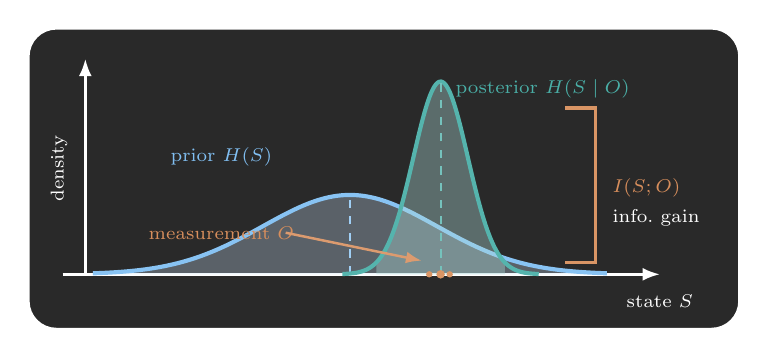
\begin{tikzpicture}[
  scale=.96, transform shape,
  every node/.style={font=\footnotesize},
  ax/.style={-{Latex[length=2.2mm]}, line width=.9pt, white!55},
  lab/.style={font=\scriptsize, text=white!85}
]
\begin{scope}[on background layer]
  \fill[black!84, rounded corners=10pt] (-4.25,-.72) rectangle (5.15,3.25);
  \draw[white!12, rounded corners=10pt, line width=.7pt]
    (-4.25,-.72) rectangle (5.15,3.25);
\end{scope}
% axes
\draw[ax] (-3.8,0) -- (4.1,0);
\draw[ax] (-3.5,0) -- (-3.5,2.85);
\node[lab] at (4.1,-0.35) {state $S$};
\node[lab, rotate=90] at (-3.85,1.4) {density};

% prior: wide, low
\fill[blue!32, opacity=0.30]
  plot[domain=-3.4:3.4, samples=140] (\x, {1.05*exp(-0.5*((\x)/1.15)^2)})
  -- (3.4,0) -- (-3.4,0) -- cycle;
\draw[blue!75, line width=1.5pt]
  plot[domain=-3.4:3.4, samples=140] (\x, {1.05*exp(-0.5*((\x)/1.15)^2)});
\draw[blue!60, dashed, line width=.7pt] (0,0) -- (0,1.05);

% posterior: narrow, tall, shifted
\fill[teal!38, opacity=0.38]
  plot[domain=0.35:2.05, samples=140] (\x, {2.55*exp(-0.5*((\x-1.2)/0.36)^2)})
  -- (2.05,0) -- (0.35,0) -- cycle;
\draw[teal!80, line width=1.5pt]
  plot[domain=-0.1:2.5, samples=140] (\x, {2.55*exp(-0.5*((\x-1.2)/0.36)^2)});
\draw[teal!65, dashed, line width=.7pt] (1.2,0) -- (1.2,2.55);

% measurement ticks on axis
\foreach \x/\s in {1.05/1.2, 1.2/1.6, 1.32/1.2}
  \fill[orange!80] (\x,0) circle (\s pt);

% labels in empty regions only
\node[lab, text=blue!80] at (-1.7,1.55) {prior $H(S)$};
\node[lab, text=teal!85] at (2.55,2.45) {posterior $H(S\mid O)$};
\node[lab, text=orange!85] at (-1.7,0.55) {measurement $O$};
\draw[orange!75, -{Latex[length=2mm]}, line width=.9pt]
  (-0.85,0.55) -- (0.95,0.18);

% information gain callout — right margin, free of curves
\draw[orange!80, line width=1.1pt]
  (2.85,2.2) -- (3.25,2.2) -- (3.25,0.15) -- (2.85,0.15);
\node[lab, text=orange!85, anchor=west] at (3.35,1.15) {$I(S;O)$};
\node[lab, text=white!60, anchor=west] at (3.35,0.75) {info.\ gain};
\end{tikzpicture}
\caption{An informative observation transforms a broad prior into a more useful
posterior. The value is not abstract certainty; it is the reduction in
uncertainty relevant to the next action.}
\label{fig:belief-update}
\end{figure}

\section{Deep Representations with Physical Structure}
\label{sec:physics}

Deep learning provides flexible representations for pixels, point clouds,
proprioception, and contact histories. Yet unconstrained representations can
use shortcuts that fail under viewpoint changes, new materials, or altered
dynamics. Physical structure offers inductive biases that improve data
efficiency and improve the meaning of latent variables.

For a learned dynamics model $f_\theta$, a physics-informed objective can
combine data fit with a residual from a known differential equation:

\begin{equation}
  \mathcal{L}(\theta) = \mathcal{L}_{\mathrm{data}}(\theta)
  + \lambda_{\mathrm{phys}}\,
  \mathbb{E}_{t}\left[\left\|
    \frac{\partial \hat{x}_\theta}{\partial t}
    - F_{\mathrm{phys}}(\hat{x}_\theta,u_t)
  \right\|^2\right].
  \label{eq:physics-loss}
\end{equation}

The same principle applies beyond explicit dynamics. SE(3)-equivariant
features respect rigid-body transformations; geometric encoders preserve
relations between points; differentiable simulators expose contact and
constraint structure; and neural operators can learn corrections to PDE or
rigid-body models. These priors do not replace learning. They restrict the
hypothesis space to functions that are easier for a robot to identify.

\begin{figure}[ht]
\centering
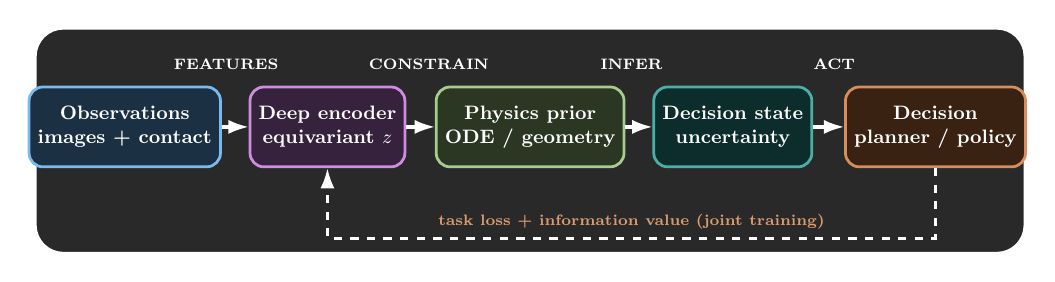
\begin{tikzpicture}[
  scale=.78, transform shape,
  every node/.style={font=\footnotesize},
  block/.style={rounded corners=5pt, draw=#1!85, fill=#1!28!black,
    text=white, align=center, minimum height=13mm, minimum width=25mm,
    line width=1pt, font=\small\bfseries, inner sep=4pt},
  arr/.style={-{Latex[length=2.6mm,width=1.8mm]}, line width=1.15pt, white!72},
  ann/.style={font=\scriptsize\bfseries, text=white!72}
]
\begin{scope}[on background layer]
  \fill[black!84, rounded corners=10pt] (-1.45,-2.05) rectangle (14.65,1.6);
  \draw[white!12, rounded corners=10pt, line width=.7pt]
    (-1.45,-2.05) rectangle (14.65,1.6);
\end{scope}
% single clean row
\node[block=blue]   (obs)    at (0,0)    {Observations\\images + contact};
\node[block=purple] (enc)    at (3.3,0)  {Deep encoder\\equivariant $z$};
\node[block=green]  (phys)   at (6.6,0)  {Physics prior\\ODE / geometry};
\node[block=teal]   (latent) at (9.9,0)  {Decision state\\uncertainty};
\node[block=orange] (policy) at (13.2,0) {Decision\\planner / policy};

\draw[arr] (obs)    -- (enc);
\draw[arr] (enc)    -- (phys);
\draw[arr] (phys)   -- (latent);
\draw[arr] (latent) -- (policy);

% labels above, clear of arrows
\node[ann] at (1.65,1.02)  {FEATURES};
\node[ann] at (4.95,1.02)  {CONSTRAIN};
\node[ann] at (8.25,1.02)  {INFER};
\node[ann] at (11.55,1.02) {ACT};

% feedback path fully below the row
\draw[arr, dashed, white!50]
  (policy.south) -- ++(0,-1.15) -| (enc.south);
\node[ann, text=orange!75] at (8.25,-1.55)
  {task loss + information value (joint training)};
\end{tikzpicture}
\caption{A hybrid perception model. Deep features capture appearance and
contact cues, while physical structure regularises the latent state passed to
the planner or controller. The decision objective can train the whole system.}
\label{fig:hybrid}
\end{figure}

\section{A Unified Learning Objective}
\label{sec:unified}

The preceding pieces suggest a training objective that scores representations
by both predictive quality and their usefulness for action. Let $Z=f_\theta(O)$
be a learned representation and $\pi_\psi$ a decision mechanism. A schematic
objective is

\begin{equation}
  \min_{\theta,\psi}\;
  \mathbb{E}\left[\mathcal{L}_{\mathrm{task}}(\pi_\psi(Z),G)
  + \alpha\,\mathcal{L}_{\mathrm{phys}}(Z)
  - \beta\,I(Z;S\mid G)\right].
  \label{eq:unified-loss}
\end{equation}

The final term is deliberately conditional on the goal. Maximising information
about every possible property is wasteful; the robot should preserve
information that changes the decision. In practice, $I(Z;S\mid G)$ can be
approximated with variational bounds, contrastive objectives, ensembles, or
uncertainty-aware world models. The physics term can be a differentiable
residual, an equivariance penalty, or a simulator consistency loss.

This view also clarifies the role of existing decision systems. A structured
planner can use a belief whose state variables carry calibrated uncertainty. An
optimisation-based controller can select trajectories that expose informative
contact modes. A learned policy can receive a latent state that separates
task-relevant ambiguity from nuisance variation. The decision mechanism
changes; the information interface remains.

\section{Discussion}
\label{sec:discussion}

Several challenges remain. Mutual information is difficult to estimate in high
dimensions, and a poor variational bound can reward representation artifacts.
Physics models are incomplete, so an overly strong residual can make the model
less accurate in regimes where the assumed equations fail. Finally, active
information gathering has a real cost: time, energy, collision risk, and
hardware wear must enter the objective alongside information value.

These limitations motivate a pragmatic combination of methods rather than a
single replacement for existing robotics stacks. Deep networks provide rich
perceptual features, physical priors improve extrapolation, information theory
identifies what uncertainty matters, and planners or controllers turn beliefs
into structured action. The most useful systems will likely compose all four.

\section{Conclusion}
\label{sec:conclusion}

Perception and decision making should not be separated by an interface that
forgets uncertainty. A robot should learn representations that preserve the
information needed to act, use physical structure to make those representations
stable, and choose observations when they have high expected decision value.
This perspective is compatible with search, optimisation, and learned policies:
it gives each of them a better, more informative belief on which to operate.

\begin{thebibliography}{9}
\bibitem{cover2006elements}
T.~M. Cover and J.~A. Thomas.
\newblock \emph{Elements of Information Theory}.
\newblock Wiley, 2006.

\bibitem{karniadakis2021physics}
G.~E. Karniadakis, I.~G. Kevrekidis, L.~Lu, P.~Perdikaris, S.~Wang, and
L.~Yang.
\newblock Physics-informed machine learning.
\newblock \emph{Nature Reviews Physics}, 3:422--440, 2021.

\bibitem{tishby2015deep}
N.~Tishby and N.~Zaslavsky.
\newblock Deep learning and the information bottleneck principle.
\newblock In \emph{IEEE Information Theory Workshop}, 2015.
\end{thebibliography}

\end{document}
